\section{Support Vector Machines}
Support vector machines are a set of supervised machine learning algorithms than can be used either for classification or regression proposed by Vapnik in 1963 \cite{VapLer63}. The main idea originates with binary classification and consists of finding an optimal hyper-plane between the data-points separating both target classes.

\subsection{Linear support vector machines}
In its primal form, the support vector machine corresponds to the following minimization problem
\begin{equation}
    \begin{aligned}
& \underset{x}{\text{minimize}} 
& & \frac{1}{2}w^Tw + C \sum_{k=1}^N \xi_k \\
& \text{subject to}
& & y_i\left[ w \cdot x_i+b \right] \geq 1-\xi_i, \; i = 1, \ldots, N \\
& 
& & \xi_i \geq 0, \; i = 1, \ldots, N.
\end{aligned}
\end{equation}
This corresponds to finding a hyper-plane defined by the vector $w$ and intercept $b$ that separates all the data-points. The minimization of $w^Tw = \norm{w}^2$ corresponds to maximizing the margin between the hyper-plane and the nearest data-points. This is the criterion used to define an unique hyper-plane as an infinity that separates the data-points correctly may exist. Indeed, the nearest data-points $x$ are on the parallel hyper-plane $w^Tx-b= \pm 1$. The distance between the margin and the nearest point is thus $1/\norm{w}$. Maximizing it means minimizing $\norm{w}$ and due to the monotony of the norm $\norm{w}^2 = w^Tw$.

Of course, it can happen that no hyper-plane is able to classify all points correctly. Slack variables $\xi_k$ are therefore introduced. The trade-off between the best possible classification of the data-points (the contribution of the slack variables) and the maximizing of the margin is controlled by the box contraint parameter $C$.

New data-points (queries) are estimated as
\begin{equation}
    \mathtt{SVM}(x) = w \cdot x + b 
\end{equation}
The classification is given by the side of the hyper-plane on which the data-point resides which corresponds to taking the sign of this estimation.

In comparison to other machine learning algorithms like neural networks for example, the SVMs present the big advantage taking the form of a convex optimization problem. But their greatest strength in my opinion is the ability to use transformations for representing a non-linear separation. Therefore, we have to to work in the dual space, where the SVM optimization problem now reformulates
\begin{equation}
    \begin{aligned}
& \underset{\alpha_i}{\text{maximize}} 
& & \sum_{i=1}^N \alpha_i - \frac12 \sum_{i,j=1}^N \alpha_i \alpha_j y_i y_j (x_i \cdot x_j) \\
& \text{subject to}
& & 0 \leq \alpha_i \leq C \; i = 1, \ldots, N \\
& 
& & \sum_{i=1}^N\alpha_i y_i = 0.
\end{aligned}
\end{equation}
and the estimation of a new data-point now becomes
\begin{equation}
    \mathtt{SVM}(x) = \sum_{i=1}^N \alpha_i y_i (x_i \cdot x) + b
\end{equation}
The dual formulation gives its name to support vector machines. A new data-point is estimated based on the other vectors from the training size and their corresponding weights. The box constraint parameter here corresponds to the maximum weight of a support vector. In the case of privacy-friendliness, support vectors are very sensitive data as they directly represent instances from the original training data-set.

\subsection{Mercer's trick and non-linear support vector machines}
The main problem of support vector machines as described above is that they are limited to linear relations between the feature elements. However, feature relations, especially in high dimension spaces require non-linear relations. Therefore, it would be interesting to map the instances into a space of higher dimension $\phi(x)$.

The feature vectors are only appearing in the form of a scalar product, which allows us to use Mercer's trick. The idea is to replace the scalar products by a kernel function $K(x_i,x_j) = \phi(x_i) \cdot \phi(x_j)$. In most kernel functions, the feature vector is mapped into a space of infinite dimension. We thereby have to consider the scalar product in a Hilbert space to keep the mathematical sense of it: $\phi(x_i) \cdot \phi(x_j) = \langle \phi(x_i), \phi(x_j) \rangle_{\mathcal{H}}$.

We can define the kernel matrix as $K_{ij} = K(x_i,x_j)$. A very interesting property of the kernel matrix is there is no need for computing the explicit transformation of each data-point as we are only interested in their scalar product. Indeed, they are never used on their own, but always in the kernel matrix. As such, one may directly compute the direct matrix. This is even more interesting as the scalar product in Hilbert spaces are practically infeasible as such. Different kernel functions are possible, that represent the scalar product of different transformations. These kernel functions rely more often on one or more hyper-parameter that has to be trained. The most common choices are
\begin{itemize}
    \item \textbf{Linear kernel function:} this corresponds to computing directly the scalar product onto the identity transformation $\phi(x_i)=x_i$ and is thus equivalent to a linear PCA analysis.
    \begin{equation}
        K(x_i,x_j) = x_i \cdot x_j
    \end{equation}
    \item \textbf{Radial basis function kernel function (RBF):} this kernel function has one hyper-parameter. At a scale factor excepted, this corresponds to the probability of the second instance given the first one with standard deviation $\sigma$. An interesting property of this kernel function is its ability to measure similarity as it converges to zero as the distance between both data-points increase and the point thus becoming more and more dissimilar. RBF are known to have excellent generalization capabilities.
    \begin{equation}
        K(x_i,x_j) = e^{\frac{-\norm{x_i-x_j}^2}{2\sigma^2}}
    \end{equation}
    \item \textbf{Polynomial kernel function:} this kernel function also has one hyper-parameter $d$. In the practice, $d=2$ is often chosen as higher order tend to overfit.
    \begin{equation}
        K(x_i,x_j) = (x_i \cdot x_j +1)^d
    \end{equation}
\end{itemize}

Due to their strong generalization power, RBF kernel generally perform better than other kernels, especially if no additional knowledge of the data is available or multi-class problems as the different classes often are often more diverse and require more generalization. In the case of intrusion detection systems, RBF kernel functions also tend to show better results \cite{Kuang2014ADetection}. Though, other kernels seem to show better results in some specific binary cases \cite{Elkhadir2016IntrusionMethods}. In our case and as we will work with multi-class classifiers, we will also opt for RBF kernel functions.

The SVM dual formulation now becomes
\begin{equation}
    \begin{aligned}
& \underset{\alpha_i}{\text{maximize}} 
& & \sum_{i=1}^N \alpha_i - \frac12 \sum_{i,j=1}^N \alpha_i \alpha_j y_i y_j K(x_i, x_j) \\
& \text{subject to}
& & 0 \leq \alpha_i \leq C \; i = 1, \ldots, N \\
& 
& & \sum_{i=1}^N\alpha_i y_i = 0.
\end{aligned}
\end{equation}
with estimation
\begin{equation}
    \mathtt{SVM}(x) = \sum_{i=1}^N \alpha_i y_i K(x_i,x) + b
\end{equation}
However, there is also a downside: we are now facing an optimization problem in the dimension of the number of input instances and not of the dimension of the feature space anymore. This means that the number of support vector will drastically increase, which is a bad scenario for our privacy-friendly models. This is one of the investigated trade-offs.


\subsection{Multi-class SVMs}
The main problem of SVM for multi-class classification is that they are not natively suited for it. Indeed, SVM return a single number representing how far the tested data-point is from the hyper-plane. SVMs are by definition created for binary classification as the whole idea behind it is to separate the feature space into two parts. The kernel trick doesn't change anything to that as it only projects the data-point into a space of higher --- often unlimited --- dimension where a new hyper-plane is searched for, but still dividing this new higher dimension space into two parts.

Ideas for classifying SVMs into different classes could be for example to put the output number into bins. However, this is a very bad idea as it would in fact suggest that all the different classes are divided by parallel hyper-planes at a distances corresponding the the range of the bins, which range could also be trained (figure~\ref{mach:svm-model-gr-1}). It almost never occurs that one hyper-plane separates two classes perfectly, the fact that $n-1$ parallel hyper-planes separate the feature space according the the $n$ different classes is even less likely. This hypothesis is much too strong and must be discarded. We therefore have to use more than one SVM and combine them.

We will present here two different ways of combining SVMs that have both been tested in the case of intrusion detection systems \cite{Kuang2014ADetection}\cite{SumaiyaThaseen2017IntrusionSVM} and produce fairly similar results although they never have been compared using exactly the same model for the rest.

The first way and the most frequent one is to create $n$ different classifiers, each for a class, and to look at which one produces the best results. 
\begin{equation}
    \underset{k}{\mathrm{arg}\,\mathrm{min}}\left\{ \mathtt{SVM}_k (x_i)   \right\}_{1 \ldots n} 
\end{equation}
where $\mathtt{SVM}_k$ represents the SVM for each class $k$. Each classifier takes as binary input, +1 for the class and -1 for all the rest data-points  (figure~\ref{mach:svm-model-1}). A way of interpreting it is looking for which SVM the data-point lies the farthest from the hyper-plane, at its good size (i.e. positive). This can be graphically observed at figure~\ref{mach:svm-model-gr-2}. This is called the \emph{one-against-all} model.

\begin{figure}[ht!]
    \centering
    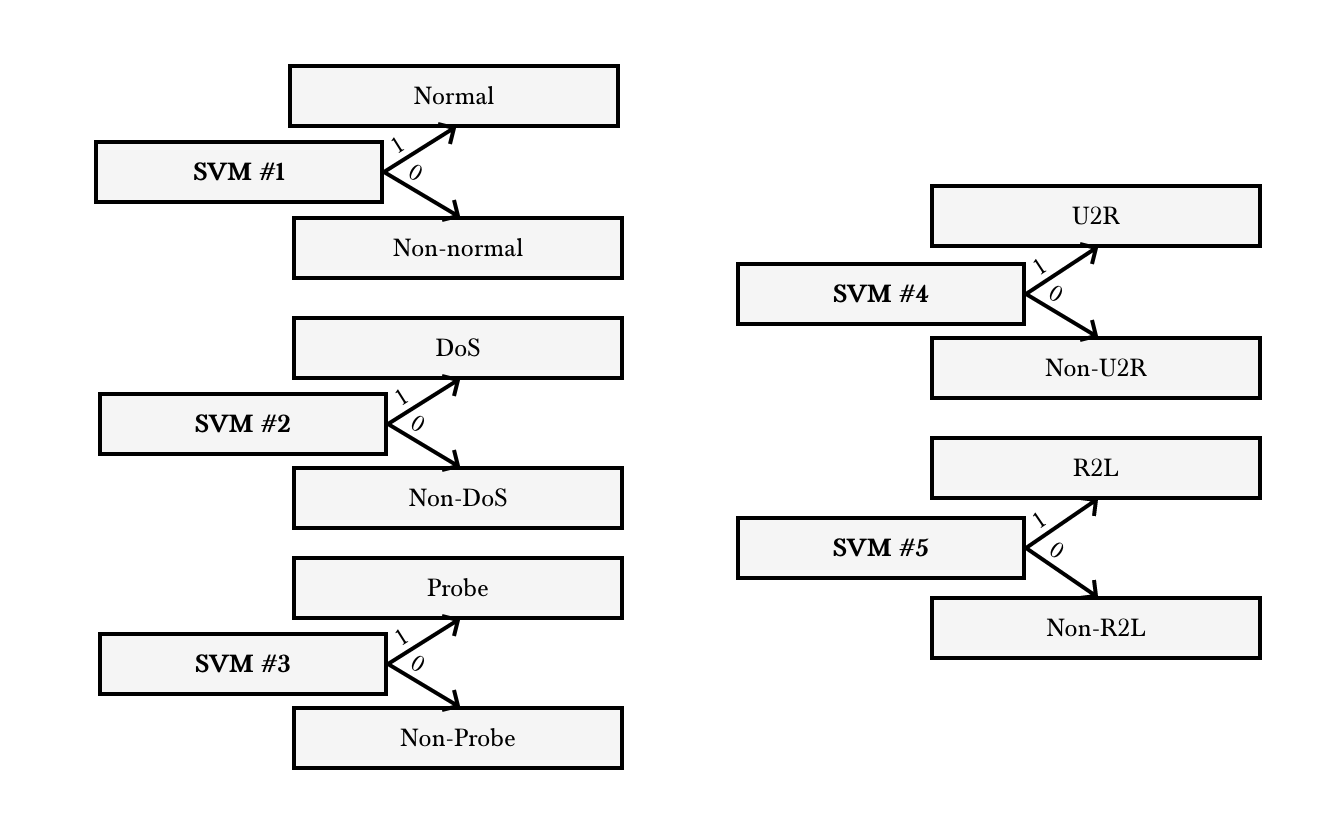
\includegraphics[width=.85\textwidth]{parts/chap-2/img-2/model-svm-1.png}
    \caption{One-against-all multi-class SVM model.} 
    \label{mach:svm-model-1}
\end{figure}

Another way of doing it is to work with successive SVMs as in figure~\ref{mach:svm-model-2} and is referred to as \emph{tree-based} models in this thesis. The first SVM is trained using one class as input versus all the others, as the first model. However the next classes are trained using one of the remaining classes versus the others remaining classes. The big advantage is that is only need $n-1$ different SVMs, which is one less compared to the previous model. Another advantage is that the last SVMs are trained one more specific data. However, the drawback is -- which is recurrent in series model --- that if one of the SVM isn't efficient, all the model is suffering. Graphically, this can be interpreted as first dividing the space with an hyper plane into two parts. One of the two parts is the subdivided into two new parts and so on (figure~\ref{mach:svm-model-gr-3}). Other tree structures are also to be considered, but this is not the scope of this thesis. We will limit ourselves to the consideration of these tree-structures in different orders. The goal of the machine-learning study of this thesis is to try to reduce the number of operations made by the evaluation of a query on the machine-learning algorithm. Computing 4 SVMs instead of 5 indeed decreases these number of computations. We thus want to investigate if this has an impact on the classification performance. A study on the comparison between the different tree-based models is a totally other subject which is not pursued here. We just limit ourselves to the different models found in the papers.

For the sake of completion, we also have to mention the existence of \emph{one-against-one} models where a binary classifier is trained for all combinations of two classes. The winning class it the one whose corresponding classifiers have the most positive outputs. However, this model needs $n_c(n_c-1)/2$ different classifiers where $n_c$ is the total number of classes, which is the opposite of the goal we are seeking.


\begin{figure}[ht!]
    \centering
    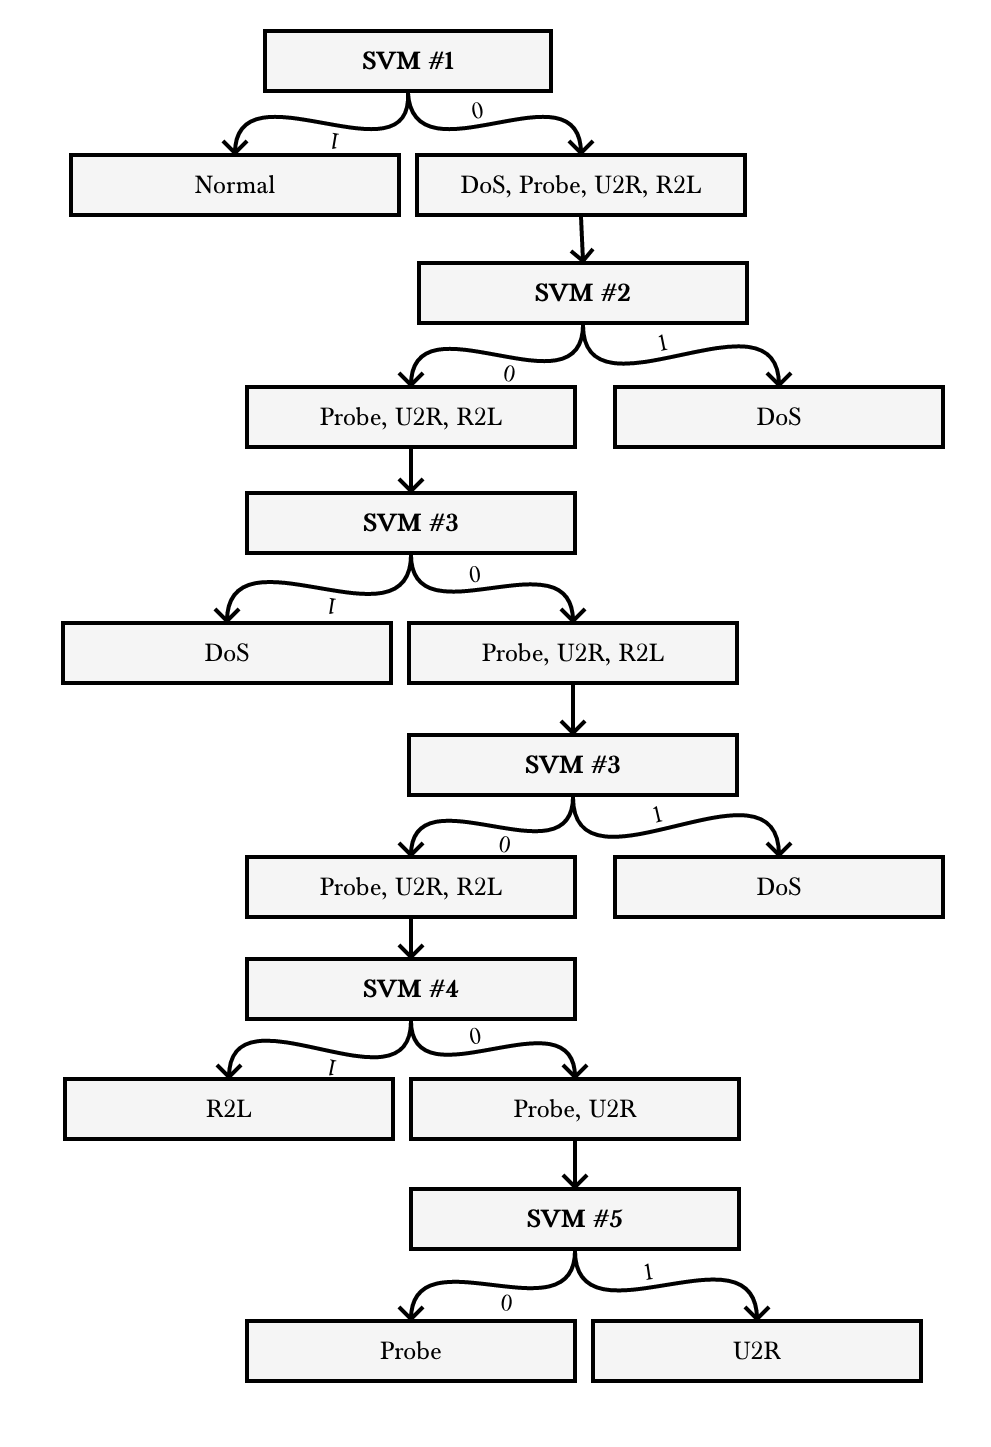
\includegraphics[width=.75\textwidth]{parts/chap-2/img-2/model-svm-2.png}
    \caption{Tree-based multi-class SVM model.} 
    \label{mach:svm-model-2}
\end{figure}

\begin{figure}
\begin{subfigure}[b]{0.32\textwidth}  
            \centering 
            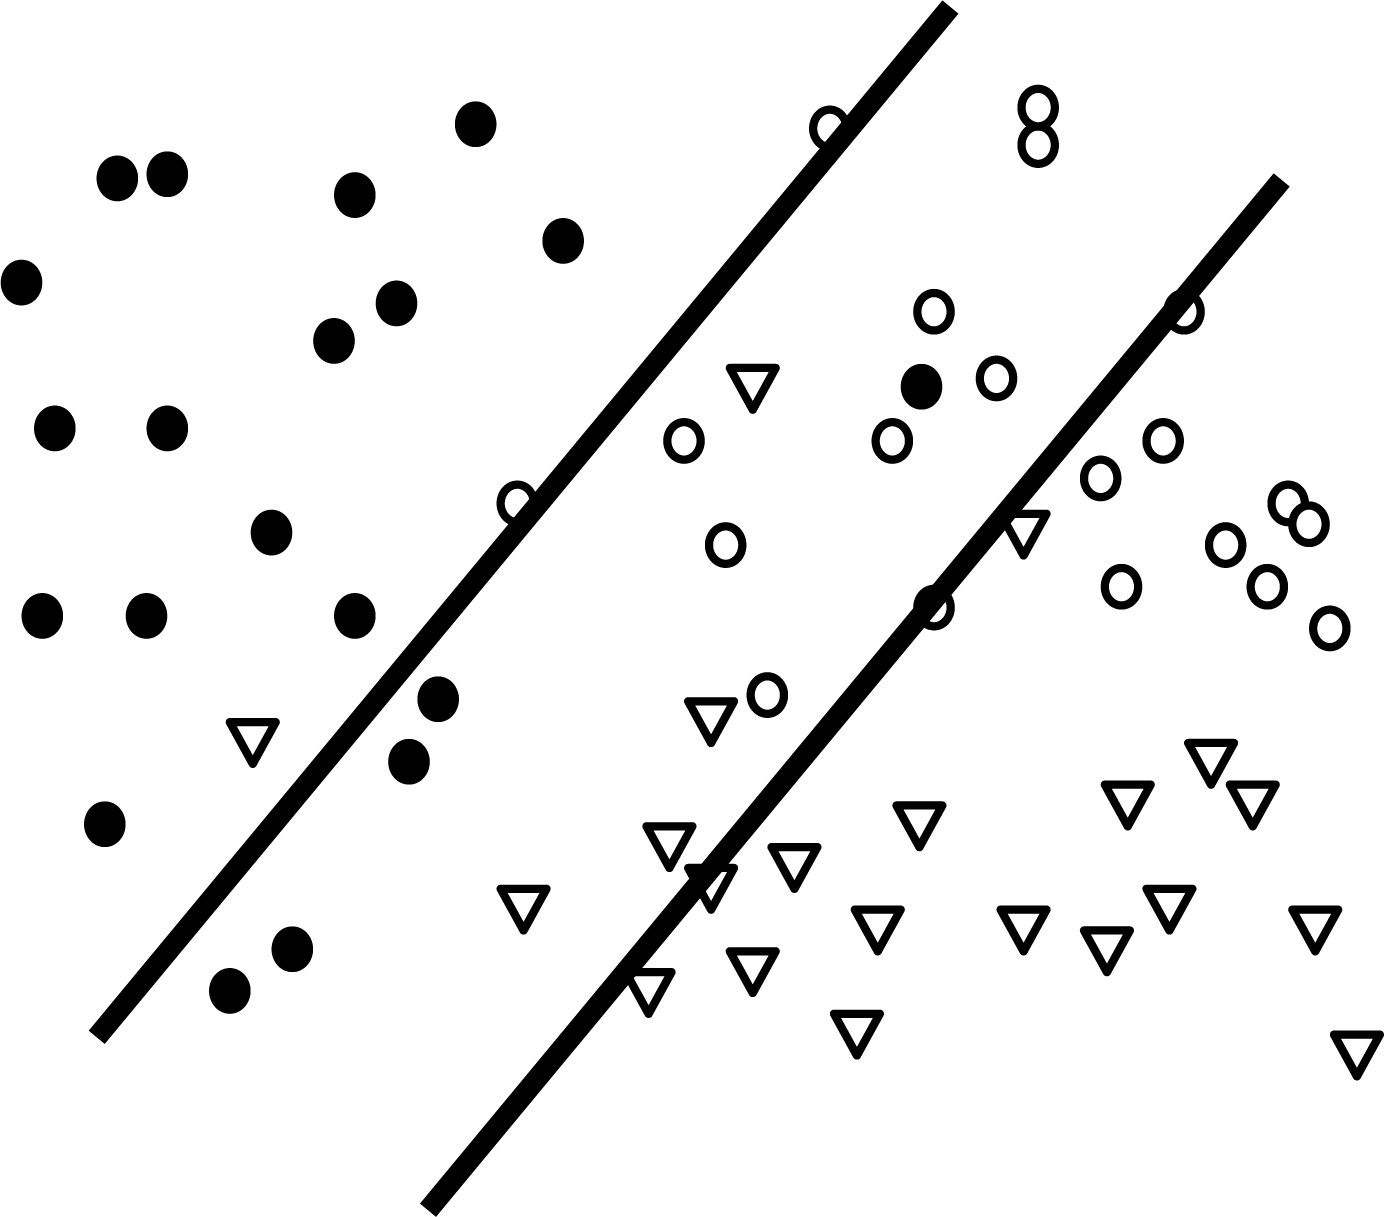
\includegraphics[width=.85\textwidth]{parts/chap-2/img-2/svm-par.png}
            \caption{Single SVM with bins.} 
            \label{mach:svm-model-gr-1}
        \end{subfigure}
        \hfill
        \begin{subfigure}[b]{0.32\textwidth}  
            \centering 
            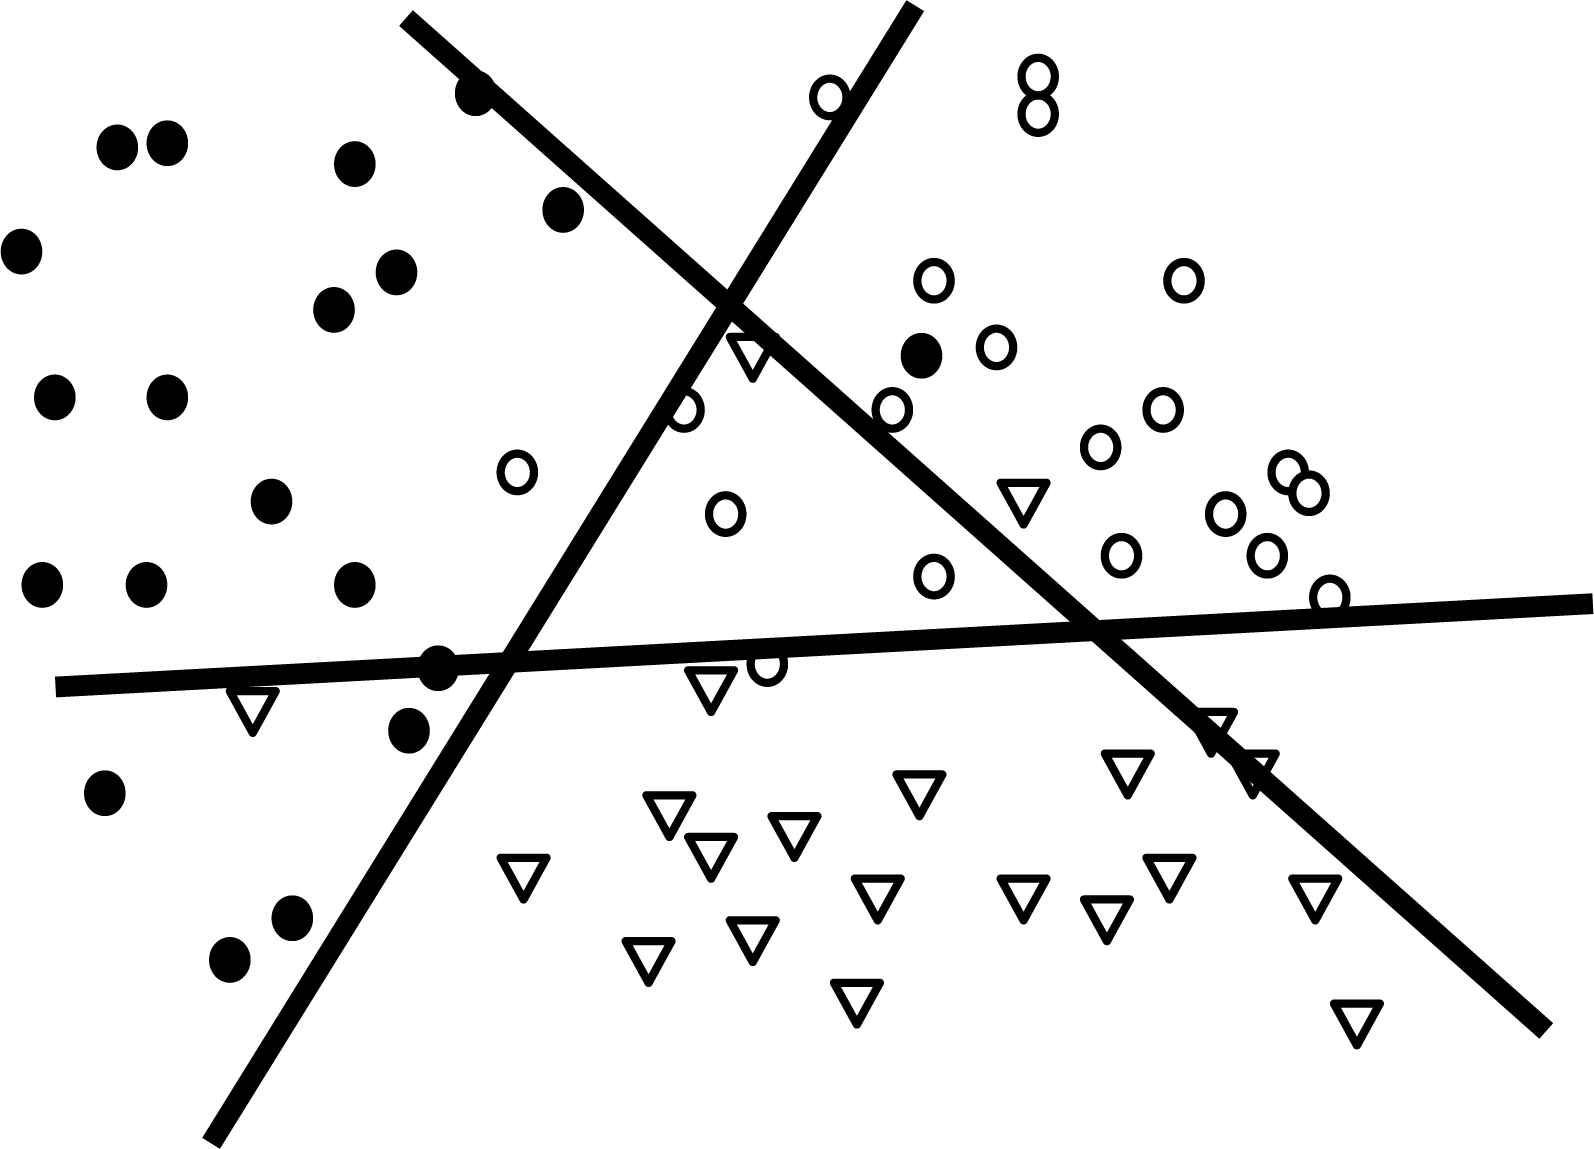
\includegraphics[width=.98\textwidth]{parts/chap-2/img-2/svm-multi.png}
            \caption{$n$ SVMs in a one-against-all model.} 
            \label{mach:svm-model-gr-2}
        \end{subfigure}
        \hfill
        \begin{subfigure}[b]{0.32\textwidth}   
            \centering 
            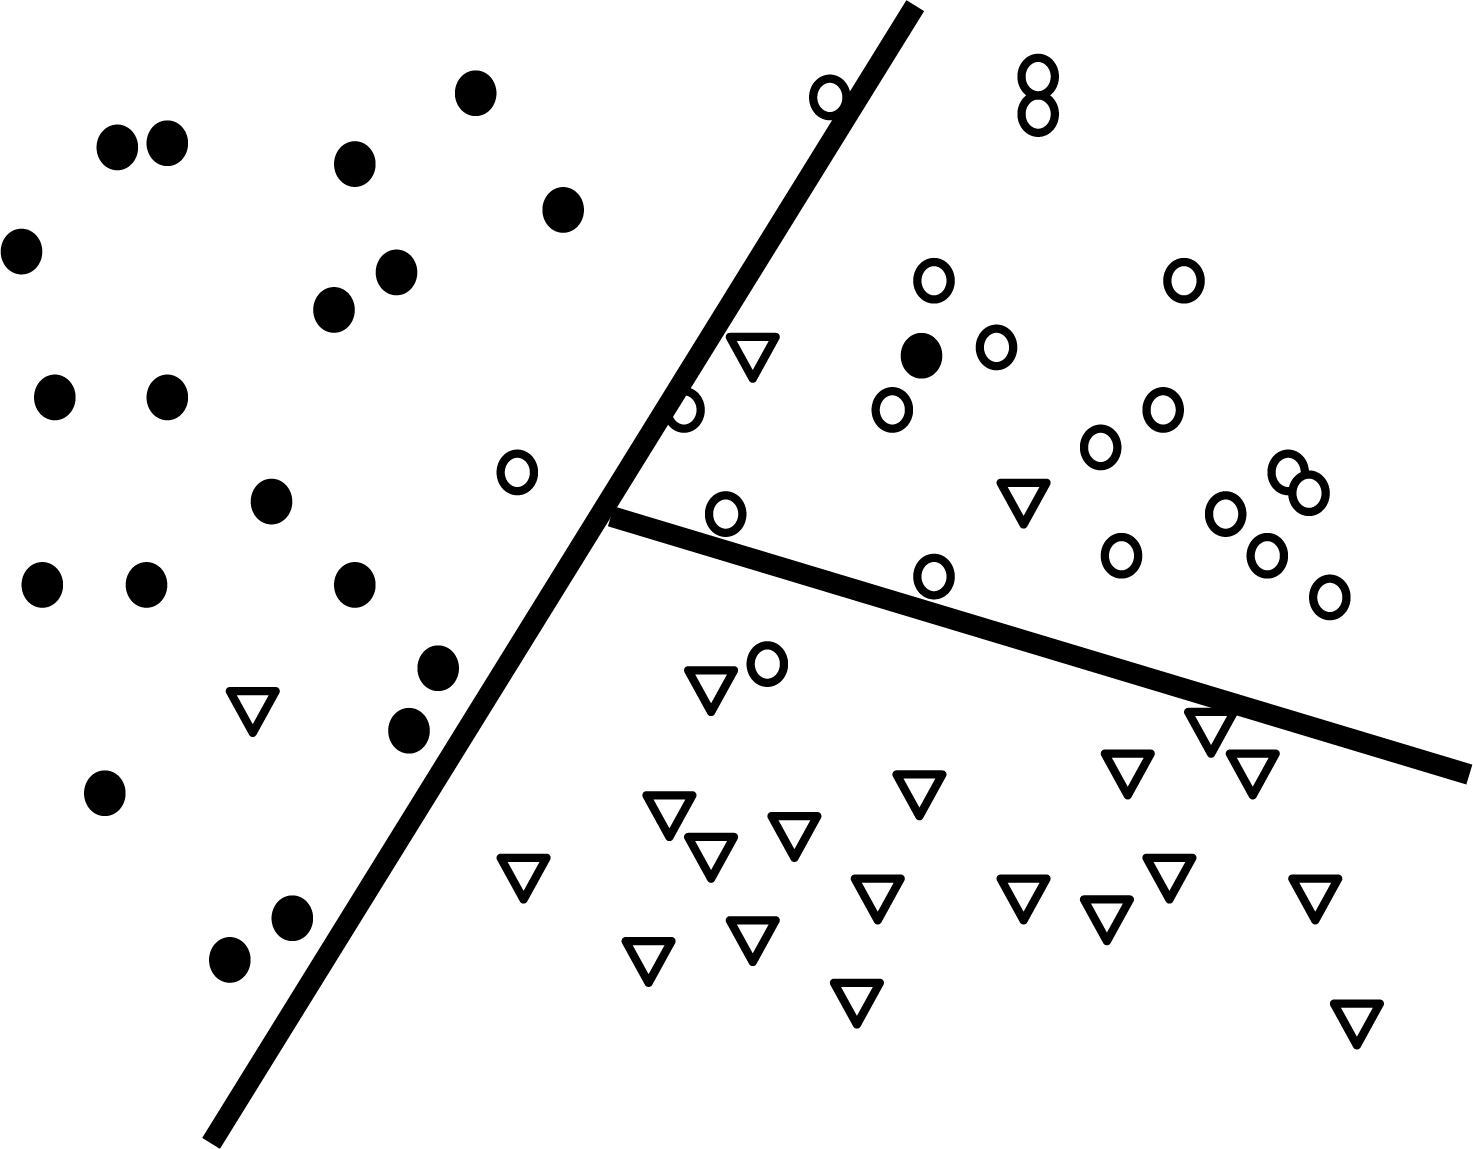
\includegraphics[width=.98\textwidth]{parts/chap-2/img-2/svm-seq.png}
            \caption{$n-1$ SVMs in a tree-based model.} 
            \label{mach:svm-model-gr-3}
        \end{subfigure}
        \caption{Comparison of different multi-class models in the feature space. In this case, there are three classes $n=3$: dots, circles and triangles.}
\end{figure}